%% LatentSky — GRL manuscript (12 publication units; full version: main_agu_advances.tex)
%% Compile on Overleaf with the official AGU template (class agujournal2019),
%% or drop agujournal2019.cls + agutexSI2019.cls into this folder.
%% Structure follows the group-meeting deck (deck/build.py): model and flow matching first,
%% then the rain decomposition (skill by scale), then the horizon; WB2 is the outlook.

\documentclass[draft]{agujournal2019}
\usepackage{url}
\usepackage{amsmath}
\usepackage{amssymb}
\usepackage{lineno}
\usepackage[inline]{trackchanges}
\usepackage{soul}
\linenumbers

\journalname{Geophysical Research Letters}

\begin{document}

\title{The Size of the Storm Sets the Horizon: a Scale-Aware Evaluation of
AI Precipitation Forecasts}
%% alt candidates:
%%  - A Scale-Aware Predictability Horizon for AI Precipitation Forecasts
%%  - How Far Ahead Can AI Predict Rain? A Scale-Aware Predictability Horizon

\authors{Sophie Abramian\affil{1}, Tim Zhou\affil{2}, Sara Shamekh\affil{2}}
\affiliation{1}{Columbia University, New York, NY, USA}
\affiliation{2}{New York University, New York, NY, USA}
\correspondingauthor{Sophie Abramian}{sophieabramian@gmail.com}

%% ===================== KEY POINTS (three, <= 140 chars each) ================
\begin{keypoints}
\item Forecasts trained on mean-square error lack small rain systems and are
too weak; generative sampling restores both
\item The detection horizon grows with system size with exponent 1.8,
against 1 for persistence; flow matching lengthens it 1.3 to 1.5 times
\item Below 60 km, rain systems are lost within about an hour, far less than
the time step of operational AI weather models
\end{keypoints}

%% ===================== ABSTRACT ============================================
\begin{abstract}
How far ahead can precipitation be predicted? The answer depends on the
size of the precipitating system. We measure this dependence in a 40-day
kilometer-scale DYAMOND simulation, with rain systems identified as
objects, matched between forecast and truth, and split into area and
intensity. A U-Net trained on squared errors predicts too few small
systems, and draws the systems it finds too large and too weak. A
flow-matching model trained on the U-Net's error restores them, at the
cost of more false alarms below $65$~km. Between $60$ and $340$~km the
detection horizon grows as a power law of size: $L^{0.97}$ for
persistence, as for advection at $8$~m\,s$^{-1}$, and $L^{1.8}$ for both
models, the flow's horizon being $1.3$ to $1.5$ times longer. Operational
AI forecasts show the same biases, and a single GenCast member corrects
them as the flow does. Below $60$~km, systems are lost within about an
hour.
\end{abstract}

\section*{Plain Language Summary}
How far ahead can rain be predicted? It depends on the rain. A monsoon rain
band hundreds of kilometers wide is still there the next day, but a small
thunderstorm may not last the next hour. To measure this, a forecast must
first contain small storms. Models trained to minimize the average error do
not: when they are uncertain, they spread the rain, and their storms are
too large and too weak. We train a second network that turns this smooth
forecast into sharp, realistic rain. We then treat every rainy area as an
object with a size and an intensity, and count how many objects of each
size a forecast finds. The sharp forecast finds more storms of every size
and gives them the right size and strength, but it also predicts more small
storms that do not occur. The time over which storms are still found grows
steeply with their size. Current AI weather models behave in the same way,
and none of them can place small storms six hours ahead.

%% ===================== 1. INTRODUCTION =====================================
\section{Introduction}

How far ahead can precipitation be predicted? The answer depends on the
process that produces the rain, and each process leaves its signature in
the size of the precipitating system. An isolated convective cell is a few
tens of kilometers wide and lives about an hour. A mesoscale convective
system, organized by its own cold pools and circulations, spans hundreds
of kilometers and lives for many hours. A monsoon rain band, tied to the
large-scale circulation, spans thousands of kilometers and persists for
days. Size is therefore a measure of the organization of convection, which
controls the intensity and the variability of tropical rain
\cite{muller2022, shamekh2023}. Each size $L$ should then have its own predictability horizon $T(L)$,
the time over which a forecast keeps track of rain systems of that size
\cite{zhang2003, hohenegger2007}. Such horizons often follow a power law,
$T \propto L^{\alpha}$, whose exponent depends on how errors grow. The
textbook example is dry turbulence: with a $k^{-5/3}$ spectrum, error
reaches a scale $L$ after the turnover times of all smaller eddies, and
$\alpha = 2/3$ \cite{lorenz1969, rotunno2008}. For our problem,
precipitation, persistence gives the reference that any forecast must
beat. It keeps each storm in place while a wind $U$ carries the real one away, so a system is
lost once it has moved by its own size: $T = L/U$, and $\alpha = 1$.

Tracking studies tie the rain of a system to its life cycle: in the tropics,
long-lived mesoscale convective systems produce most of the extreme rain
\cite{roca2020}, and each precipitating phenomenon has its own scales in
space and time \cite{prein2023}. These studies follow systems above a
size or duration threshold \cite{fiolleau2013, feng2023, feng2025}. Across
all scales, from single cells to mesoscale systems, and for the AI models
that now forecast them, the exponent of the horizon has not been measured.

AI weather models forecast precipitation, but not scale by scale. They
are trained on the ERA5 reanalysis at $0.25^{\circ}$ to step the
atmospheric state forward by $6$ or $12$~h \cite{lam2023, chen2023,
price2025}, and their rain is the reanalysis rain: produced by a
convection scheme, not observed, and without convective cells smaller than
the grid. Deterministic models such as GraphCast and FuXi learn rain by
minimizing a mean-square error; FourCastNet diagnoses it with a separate
network \cite{pathak2022}, and we note in passing that Pangu-Weather does
not \cite{bi2023}. A model trained on mean-square error
predicts the mean of all futures compatible with its inputs. Like an
ensemble mean, this forecast is smooth, with rain areas too wide and
intensities too weak, and grid-point scores reward it \cite{ravuri2021}.
Generative models produce sharp members instead: by diffusion in GenCast
\cite{price2025}, by a perturbed network trained on the continuous ranked
probability score in FGN \cite{alet2025}, or by flow matching, a more
direct path from noise to data \cite{lipman2023, liu2023}. Yet these
models leave precipitation out of their main results, and radar
nowcasting models report skill per rain threshold, not per scale
\cite{andrychowicz2023, sarabia2025}. To our knowledge, the precipitation
of AI forecasts has not been evaluated system by system.

Here we ask three questions. How can a forecast produce realistic rain at
every scale? How is its skill distributed across scales? What horizon does
each scale have? Global kilometer-scale simulations provide the data to
answer them \cite{stevens2019, satoh2019}: they resolve deep convection,
from isolated cells to mesoscale systems, every $15$~min. On a 40-day
DYAMOND simulation we train a deterministic U-Net and a flow-matching
model that starts from the U-Net forecast. Both receive the current rain,
so persistence is nested in both. The models are small: a controlled
experiment, not a competitor to operational systems. The
evaluation, which matches rain objects between forecast and truth, applies
to any forecast that produces a rain field, and we apply it to three AI
models from WeatherBench~2 \cite{lam2023, chen2023, price2025, rasp2024}.

%% ===================== 2. DATA AND METHODS =================================
\section{Data and Methods}\label{sec:methods}

\subsection{Kilometer-scale data}\label{sec:data}

\begin{figure}
\centering
\makebox[\textwidth][c]{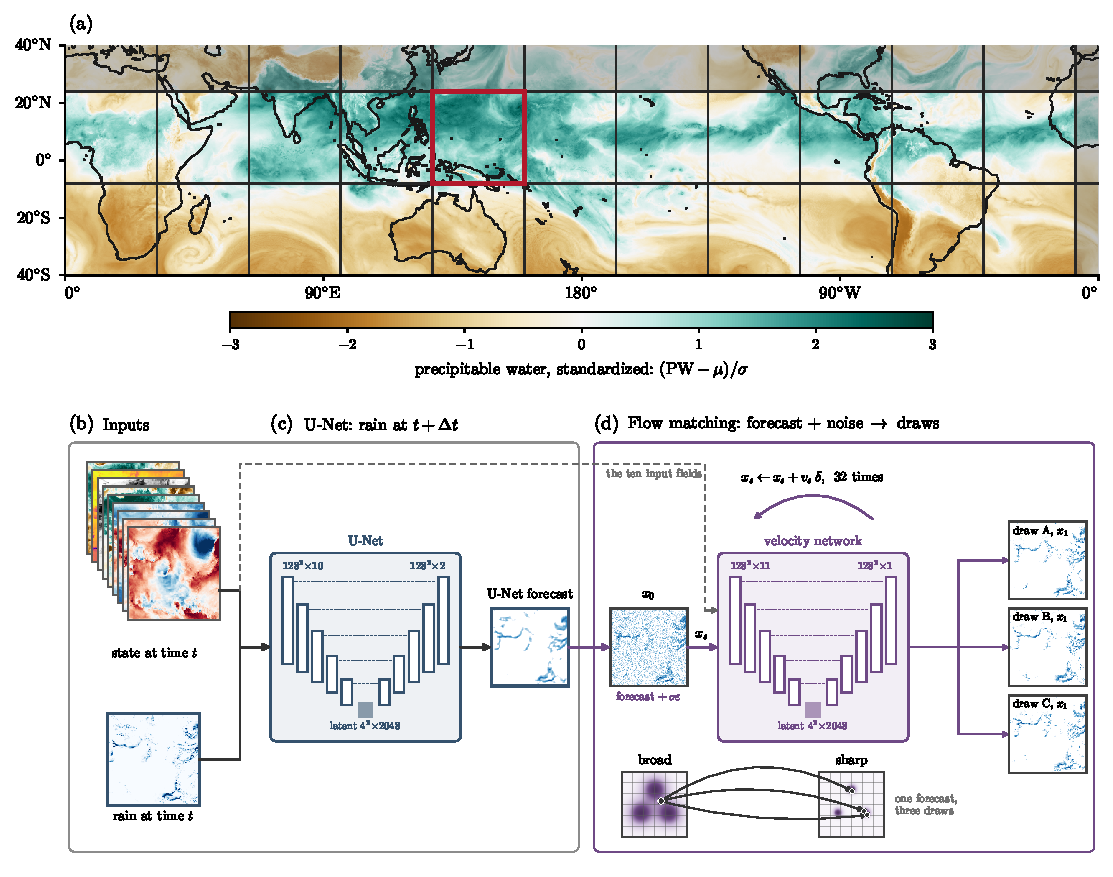
\includegraphics{figures/fig1_overview.pdf}}
\caption{Data and forecast pipeline. (a) Standardized precipitable water on
one $15$-min frame of the DYAMOND MPAS record; black lines show the
$2 \times 11$ blocks of $128 \times 128$ pixels, and the red box marks the example block of panels (b)--(d) and
Figure~\ref{fig:pairs}. (b) The ten input fields at time $t$. (c) The
U-Net, which maps them to the rain at $t + \Delta t$. (d) Flow matching at
a $3$~h lead: the forecast plus noise is carried to a sharp field in $32$
steps of the velocity network, which also receives the input fields
(dashed); three noise fields give three draws. Rain maps share one logarithmic color scale.}
\label{fig:data}
\end{figure}

We use the DYAMOND MPAS-Atmosphere simulation \cite{stevens2019}, a global
storm-resolving run at ${\sim}3.8$~km with output every $15$~min over
40 days of boreal summer.
MPAS produces more tropical mesoscale convective systems than are observed
\cite{feng2023, feng2025}, so the horizons below are those of a simulated
atmosphere. We average the fields onto a regular $0.25^{\circ}$ grid
(${\approx}28$~km) over $40^{\circ}$S--$40^{\circ}$N and divide each frame
into $22$ blocks of $128 \times 128$ pixels (Figure~\ref{fig:data}a). The
data are split by block-day: the $880$ block-days are shuffled and divided
into $616$ for training, $132$ for validation, and $132$ for testing. No
pixel, and no $15$-min autocorrelation at a given location, is shared
between the sets (Text~S1).

The inputs are ten fields at time $t$: precipitable water, 2-m
temperature, outgoing longwave radiation, moist static energy and both
horizontal wind components at $850$ and $500$~hPa, and the rain at $t$
(Figure~\ref{fig:data}b). The target is the rain accumulated over $15$~min
at $t + \Delta t$, for $\Delta t = 0.25, 0.5, 1, 2, 3$, and $6$~h. We
train a separate U-Net and a separate flow for each lead, twelve models
in all. Each predicts the rain at its lead directly from the state at $t$,
without stepping through shorter leads.

\subsection{Models}\label{sec:unet}

The deterministic model is a U-Net, a standard encoder--decoder of
$125$~M parameters with two outputs, the rain $\hat{R}$ and a wet/dry
field $\hat{m}$ (Figure~\ref{fig:data}c; Text~S2). Its loss has three
terms,
\begin{equation}
\mathcal{L} =
\underbrace{\frac{1}{|\mathcal{M}|}\sum_{i \in \mathcal{M}}
  \big(\hat{R}_i - R_i\big)^2}_{\text{intensity}}
\;+\;
\underbrace{\mathrm{BCE}\big(\hat{m},\, \mathbf{1}[R > 0]\big)}_{\text{where it rains}}
\;+\; 0.25\,
\underbrace{\frac{1}{6}\sum_{k=1}^{6}
  \big\| \bar{f}_k(\hat{R}) - \bar{f}_k(R) \big\|^2}_{\text{tolerance to shifts}} ,
\label{eq:loss}
\end{equation}
where $R$ is the true rain, $\mathcal{M}$ the set of pixels where it is
wet, BCE the binary cross-entropy, and $\bar{f}_k$ the fraction of wet
pixels in windows of $1$ to $33$ pixels ($28$ to $920$~km). The first
term produces high rain values: computed only where the truth is wet, it
is not dominated by the many dry pixels, which would push the model toward
weak rain everywhere. The second term teaches the spatial pattern of the
rain, which pixels are wet and which are dry. The third is gentle with
shifts: comparing coarse-grained fields, it penalizes a system displaced
by a few pixels much less than a missing one.

Even with this loss, the U-Net is trained on squared errors and predicts
the conditional mean of the rain. When the position of a storm is
uncertain, its rain is spread over all possible positions and its
intensity is reduced. The forecast places the rain correctly but is too
smooth.

The generative model uses flow matching \cite{lipman2023, liu2023} to
recover the sharpness lost by averaging. It moves the U-Net forecast, in
small steps, toward a sharp rain field consistent with the inputs. During
training, each U-Net forecast $x_0$ is paired with the truth $x_1$ it was
trying to predict, and the two are joined by a straight line,
\begin{equation}
x_s = (1 - s)\,x_0 + s\,x_1, \qquad 0 \le s \le 1 .
\label{eq:line}
\end{equation}
A second U-Net, the velocity network, receives a field on this line and
the ten input fields, and learns the direction toward the truth,
$x_1 - x_0$. From many such pairs, it learns how real rain differs from a
smooth forecast: more concentrated, more intense, and organized in cells.

To produce a forecast, the model starts from the U-Net output and follows
the learned direction for $32$ steps (Figure~\ref{fig:data}d). A small
noise is added to the starting field, with an amplitude equal to the
U-Net's error at that lead. This noise selects one of the futures
compatible with the inputs. Different noise gives different draws, all
sharp and all consistent with the same inputs. A diffusion alternative is
discussed in Text~S3. We score each draw separately
and never the average of draws, since that average is again a smooth mean.

\subsection{Evaluation: systems and their matching}
\label{sec:evaluation}

In the truth and in each forecast, a system is an 8-connected set of pixels
with rain above $0.1$~mm per $15$~min. Each system has an area $A$, a mean
intensity $\rho$, a total rain $P$, and a size $L$:
\begin{equation}
P = \rho\,A, \qquad L = \sqrt{A}.
\label{eq:PrhoA}
\end{equation}
Within each frame, truth and forecast systems are paired by intersection
over union (IoU), in decreasing order of IoU, each system at most once,
down to $\mathrm{IoU} = 0.1$. A truth system without a partner is missed,
and a forecast system without a partner is a false alarm. In each size
band we compute the probability of detection (POD) over truth systems and
the false-alarm ratio (FAR) over forecast systems. For a matched pair, the
rain error splits exactly into an area and an intensity contribution,
\begin{equation}
\mathrm{d}\ln P = \mathrm{d}\ln A + \mathrm{d}\ln\rho,
\label{eq:decomp}
\end{equation}
with $\mathrm{d}\ln A = \ln(A_{\mathrm{fc}}/A_{\mathrm{truth}})$, and
similarly for $\rho$. The horizon $\tau(L)$ of a size band is the
e-folding time of its POD over the six leads, and the power law
$T(L) \propto L^{\alpha}$ is fitted to $\tau$ between $59$ and $336$~km
(Text~S4).

Persistence, the rain at $t$ used as the forecast for $t + \Delta t$, is
evaluated in the same way. It is a strong reference for
detection, because a long-lived system still overlaps its earlier position
at $\mathrm{IoU} \ge 0.1$. The segmentation is kept simple so that it
applies to any rain field; its sensitivities are in Text~S5.

%% ===================== 3. RESULTS ==========================================
\section{Results}\label{sec:results}


\subsection{Small systems are missing, not misplaced}\label{sec:res-scales}

\begin{figure}
\centering
\makebox[\textwidth][c]{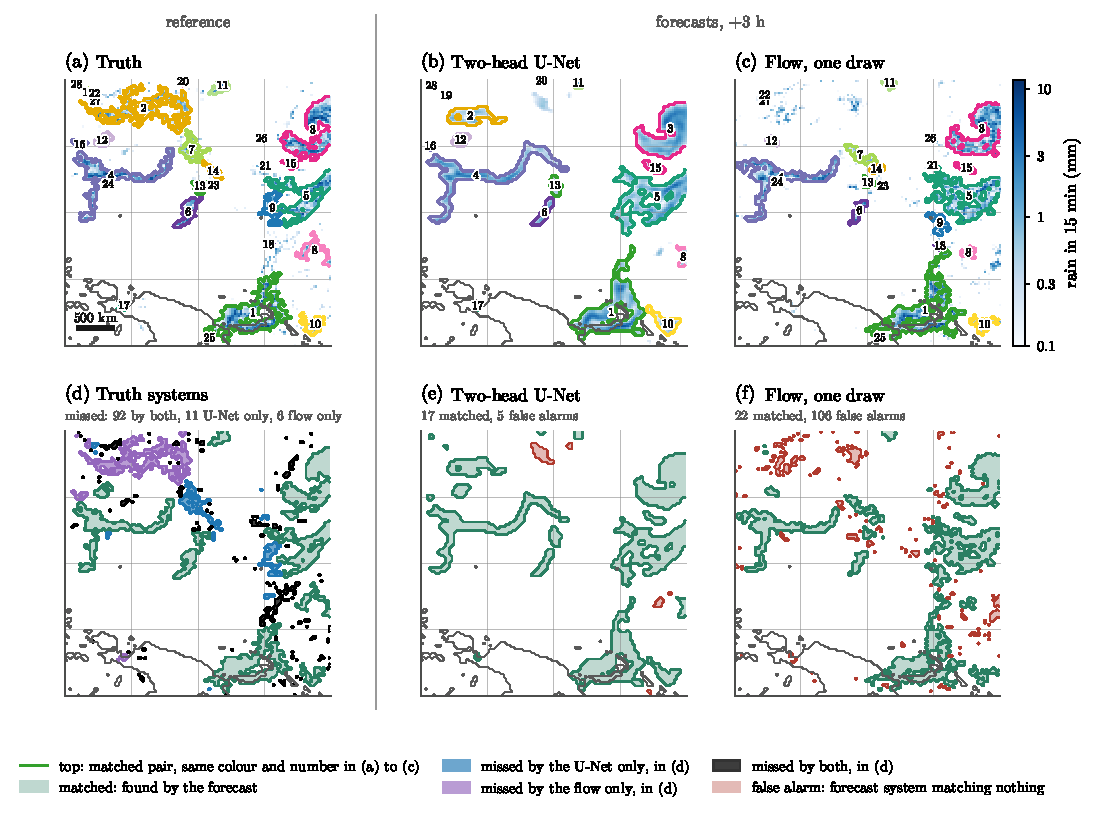
\includegraphics{figures/fig3_pairs.pdf}}
\caption{Object detection and matching on the example block at a $3$~h
lead. (a--c) Rain in the truth, the U-Net forecast, and one flow draw,
with matched systems outlined. (d) The $120$ truth systems by outcome:
found by both models (green), missed by the U-Net only (blue), by the flow
only (purple), or by both (black). (e, f) Matched systems (green) and
false alarms (red) of the U-Net and of the flow draw.}
\label{fig:pairs}
\end{figure}

Figure~\ref{fig:pairs} shows what the forecasts draw on the example block
of Figure~\ref{fig:data}a at $+3$~h. The top row gives the rain in the
truth and the two forecasts (a--c). A truth system found by a forecast
keeps the same color and number in every panel; systems found by neither
model have no outline. The bottom row sorts the systems by outcome
(d--f).

The truth contains $120$ systems. The U-Net predicts $22$, smooth and with
weak peaks, and matches $17$. The flow draw has cells and intensities like
the truth's, matches $22$, and produces $106$ false alarms against $5$ for
the U-Net. The $92$ systems found by neither model are the smallest. The
U-Net misses them mainly because it does not produce them: over the test
record, it produces $0.04$ to $0.5$ times the number of truth systems
below $120$~km and $2.4$ times too many above $600$~km, while the flow
produces $0.85$ to $1.1$ times at every size. Over the test record,
Figure~\ref{fig:decomp} gives the area and intensity of all matched
systems at $+3$~h (Section~\ref{sec:res-decomp}), and
Figure~\ref{fig:horizon} gives their detection and false alarms by size
(a, b) and, from all six leads, the decay of detection with time (c, d;
Section~\ref{sec:res-horizon}).

\subsection{The flow removes the too-large, too-weak bias}\label{sec:res-decomp}

\begin{figure}
\centering
\makebox[\textwidth][c]{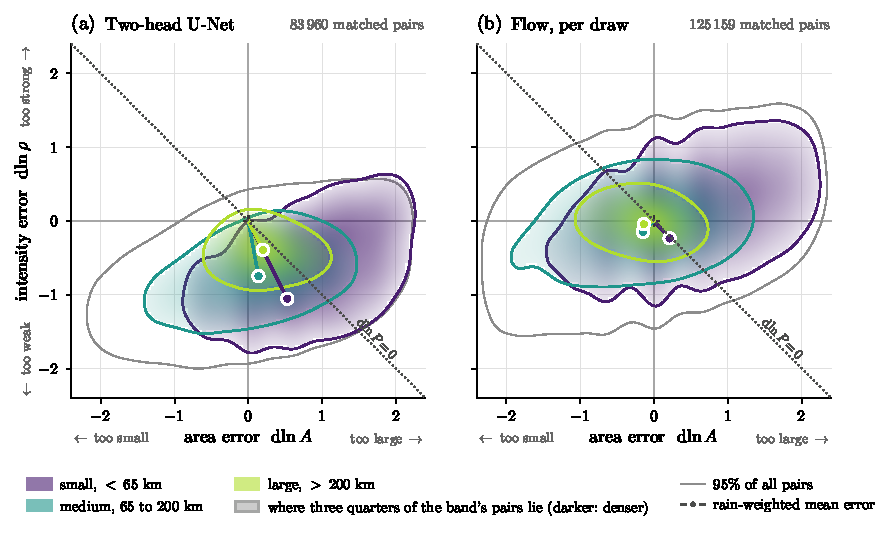
\includegraphics{figures/fig4_decomp.pdf}}
\caption{Area and intensity errors of the matched systems at a $3$~h lead
over the test record, for (a) the U-Net ($83{,}960$ pairs) and (b) one
flow draw ($125{,}159$ pairs). Shaded regions hold $75\%$ of the pairs of
each size band, darker where denser; dots mark the rain-weighted mean
error of each band; the grey outline holds $95\%$ of all pairs.}
\label{fig:decomp}
\end{figure}

Once a system is found, how well is it drawn? Each matched pair is a point
in the plane of area error $\mathrm{d}\ln A$ and intensity error
$\mathrm{d}\ln\rho$ (Figure~\ref{fig:decomp}). A perfect system sits at
the origin; on the dotted diagonal, the rain is right but spread over the
wrong area.

The U-Net's systems are too large and too weak at every size
(Figure~\ref{fig:decomp}a). Below $65$~km they are $1.7$ times too large
and three times too weak ($\mathrm{d}\ln A = +0.53$,
$\mathrm{d}\ln\rho = -1.05$); between $65$ and $200$~km, $1.15$ times too
large and twice too weak ($+0.14$, $-0.75$); above $200$~km, $1.2$ times
too large and $1.5$ times too weak ($+0.20$, $-0.39$). This is what
averaging over uncertain positions does: the rain of a system is spread
over every place it might be, so its area grows and its intensity drops.
The bias is largest for small systems, whose position is the most
uncertain relative to their size.

The flow removes this bias (Figure~\ref{fig:decomp}b). Its systems are
within $25\%$ of the truth in area and in intensity at every size (mean
errors $(+0.21, -0.24)$, $(-0.15, -0.15)$, and $(-0.14, -0.04)$), and the
three distributions are centered on the origin. The remaining $+0.21$ in
area for small systems is about one pixel: adding one pixel to a
two-pixel system already gives $+0.4$ in $\ln A$.

\subsection{Detection and its horizon grow with size}\label{sec:res-horizon}

\begin{figure}
\centering
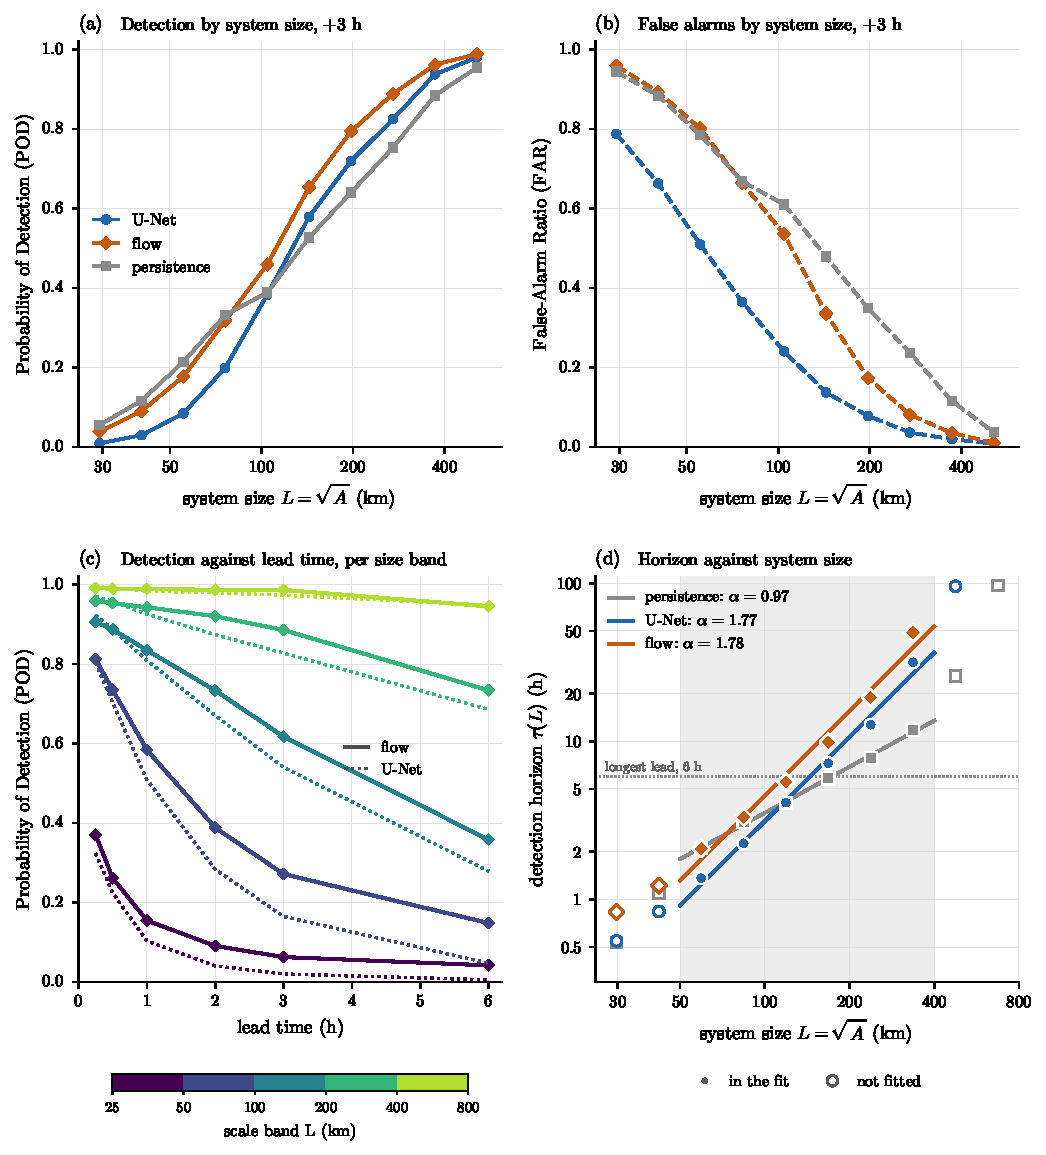
\includegraphics[width=\textwidth]{figures/fig5_horizon.pdf}
\caption{Detection by system size and the detection horizon over the test
record. (a) Probability of
detection and (b) false-alarm ratio against system size $L$ at a $3$~h
lead, for the U-Net, one flow draw, and persistence. (c) Probability of
detection against lead in five size bands (solid, flow; dotted, U-Net).
(d) Detection horizon $\tau(L)$ with power-law fits over the shaded bands
from $59$ to $336$~km; hollow markers are not fitted, and the dotted line
marks the longest lead.}
\label{fig:horizon}
\end{figure}

Detection increases with size for every forecast
(Figure~\ref{fig:horizon}a), from $0.04$ at $30$~km to $0.98$ at $480$~km
for the flow. The flow detects more than the U-Net in every band ($0.79$
against $0.72$ at $190$~km, $0.078$ against $0.028$ below $65$~km) and
produces more false alarms (Figure~\ref{fig:horizon}b; $0.92$ against
$0.64$ below $65$~km, $0.17$ against $0.08$ at $190$~km). Below $70$~km,
persistence detects more than the flow, because long-lived systems still
overlap their earlier positions, but it has the highest false-alarm ratio
at every size.

Across the six leads, each forecast by its own models, detection decays
nearly exponentially, faster for small systems
(Figure~\ref{fig:horizon}c). For the flow, the horizon $\tau$ is $0.8$~h
at $30$~km, $2.1$~h at $60$~km, $10$~h at $170$~km, and $49$~h at
$340$~km (Figure~\ref{fig:horizon}d); for the U-Net it is $0.55$, $1.4$,
$7.3$, and $32$~h.

Between $59$ and $336$~km the three horizons follow power laws.
Persistence has $\alpha = 0.97 \pm 0.07$ (95\% interval), with $L/\tau$
between $7.5$ and $8.4$~m\,s$^{-1}$ in all six bands: it loses a system
once the system has moved by its own size at about $8$~m\,s$^{-1}$, the
advective limit. The U-Net and the flow share a steeper exponent,
$1.77 \pm 0.23$ and $1.78 \pm 0.33$. The flow multiplies the horizon by
$1.3$ to $1.5$ at every size and leaves the exponent unchanged. Their gain over persistence grows with size: the U-Net falls below persistence up to about $100$~km, while the
flow is at or above it in every band ($0.83$ against $0.53$~h at $30$~km,
$9.9$ against $5.8$~h at $170$~km). Below $59$~km, all three forecasts
lose systems within $0.5$ to $1.2$~h, before the wind has moved them by
their own size: these one- or two-pixel systems end before they are
displaced.

\subsection{Operational AI forecasts share the same biases}\label{sec:res-wb2}

\begin{figure}
\centering
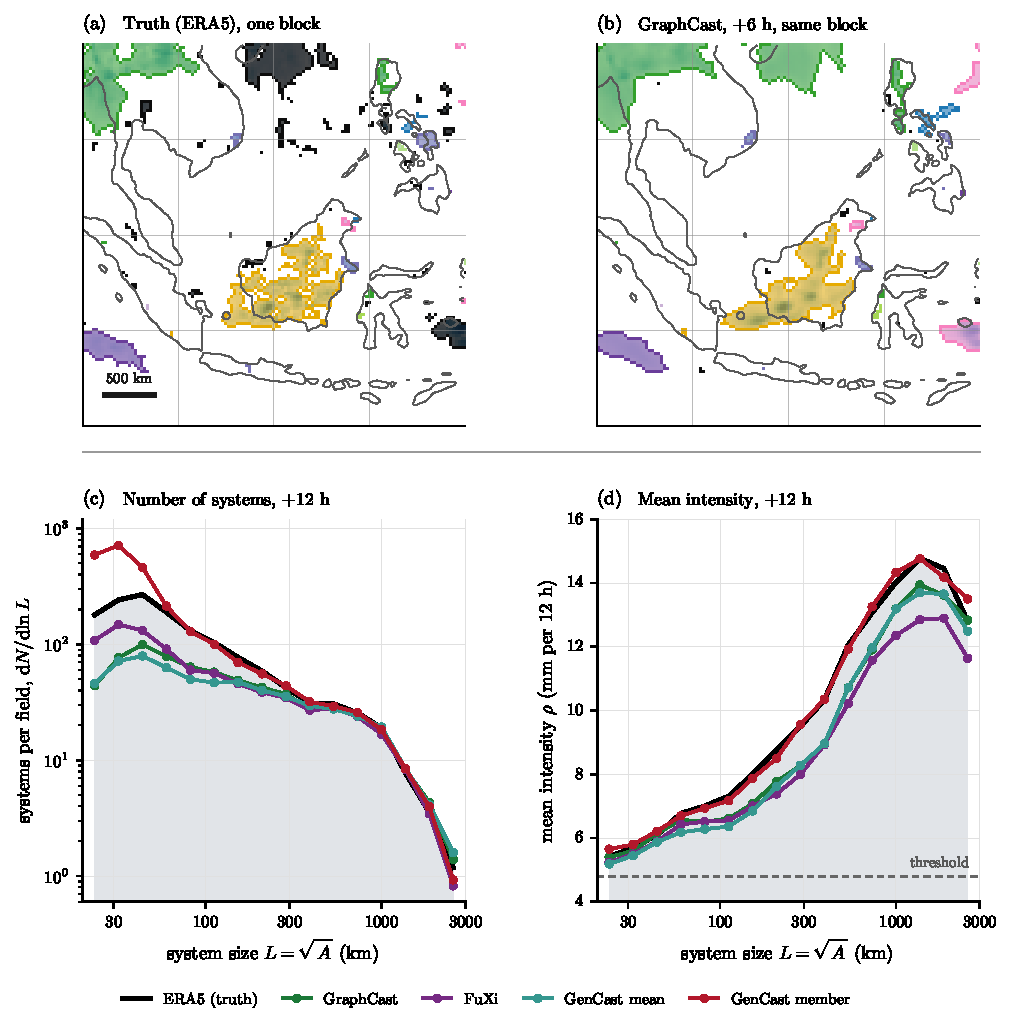
\includegraphics[width=\textwidth]{figures/fig6_wb2.pdf}
\caption{The evaluation applied to WeatherBench~2. (a, b) Object matching
for GraphCast at a $6$~h lead against ERA5 on one block of the Maritime
Continent, valid 2020-08-15 06 UTC; matched pairs share a color, and the
missed truth systems (a) and false alarms (b) are black. (c) Number of
systems per field and (d) mean intensity of the systems of each size,
for ERA5 (black) and the WeatherBench~2 models at a $12$~h lead,
pooled over August 2020 ($62$ initializations). Systems exceed $2.4$~mm
per $6$~h, the rate of the kilometer-scale threshold.}
\label{fig:wb2}
\end{figure}

We apply the same evaluation to GraphCast, FuXi, and GenCast from
WeatherBench~2, against ERA5 over the same belt, with the rain threshold
converted to the same rate (Figure~\ref{fig:wb2}a,b). Data, resolution,
and leads differ from ours, so we do not rank the two sets.

The operational models reproduce the behavior of the U-Net and the flow.
First, the mean forecasts lack small systems (Figure~\ref{fig:wb2}c).
Below $100$~km, GraphCast, FuXi, and the GenCast ensemble mean produce one
third to one half of the systems in ERA5, while above $300$~km all models
have the right number. A single GenCast member has the right number from
$80$~km upward and three times too many at $30$~km, where it fragments
rain areas (Text~S5). Second, the mean forecasts are too weak
(Figure~\ref{fig:wb2}d). In ERA5, intensity increases with size, from
$5$~mm per $12$~h at $30$~km to $14$~mm at $1{,}000$~km. Between $100$ and
$700$~km, GraphCast, FuXi, and the GenCast mean are $10$ to $15\%$ weaker,
while the GenCast member matches ERA5 at every size; matched systems give
the same result (Figure~S4). Third, detection depends on size: below
$60$~km every model detects $13\%$ of the systems or fewer at $+6$ and
$+12$~h (Figure~S5).



%% ===================== 4. DISCUSSION =======================================
\section{Discussion and conclusions}\label{sec:discussion}

We measured how far ahead rain systems can be predicted as a function of
their size. Between $60$ and $340$~km the detection
horizon follows a scaling law, $T \propto L^{\alpha}$. Persistence matches
the advective prediction, $\alpha = 0.97$ (Section~\ref{sec:res-horizon}). The trained models are steeper, $\alpha \approx 1.8$. They capture
the advection, which is why they outperform persistence, more so for large
systems. What then limits detection is the life cycle: a system is lost
when it decays, or when a new one forms unpredicted. Below $59$~km this
limit is reached first; above, it grows faster with size than the
advective bound.

For AI weather models, two conclusions follow. First, a large part of the
small-scale rain missing from mean-square forecasts is lost to the
training objective, not to a lack of information. A generative model
trained on the forecast's own error recovers it at every scale, at a
measured false-alarm cost, and GenCast members,
but not their mean, already do the same. Second, this is not enough for
the smallest systems. Their horizon, $0.8$~h at $30$~km for the flow, is
shorter than the time step of operational models, so progress below
${\sim}60$~km requires both kilometer-scale training data and forecast
steps shorter than one hour. Precipitation is therefore a test of how much
an AI model has learned about convection: producing rain systems of the
right number, size, and intensity at every scale, and sampling their
variations rather than averaging them, requires representing convection
and its stochasticity \cite{shamekh2023}.

Three extensions follow. Tracking systems through their life cycle
\cite{fiolleau2013, feng2023} would give the rain anomaly from initiation
to decay and separate displacement errors from errors in initiation and
decay. Repeating the analysis across the DYAMOND models \cite{feng2025}
would separate properties of the atmosphere from those of MPAS, which
overestimates mesoscale convective systems. Finally, the scale at which
skill is lost points AI models to the process they miss: initiation for
isolated cells, organization for mesoscale systems. Conditioning detection
on the large-scale forcing, such as ascent or moisture convergence, would
show whether a forecast is right mainly when the dynamics are strong, and
whether the extremes it misses develop under weak forcing.

\section{Open Research}
The DYAMOND MPAS output is available through the DYAMOND initiative
\cite{stevens2019}; the regridded $0.25^{\circ}$ tropical-belt fields, the
trained model checkpoints, and the full matched-system tables that underlie
every figure will be archived with a DOI upon acceptance
%% TODO: mint the archive (Zenodo or NCAR GDEX) before submission
. The WeatherBench~2 forecasts (GraphCast, FuXi, GenCast) and the ERA5
verification fields are publicly available from the WeatherBench~2 cloud
archive \cite{rasp2024}. All analysis and figure code --- the object
detection, matching, and $\rho A$ decomposition, the training and sampling
code for both models, and one script per figure --- is available at
%% TODO: public repository URL
the project repository.

\acknowledgments
Computing resources were provided by the NSF National Center for
Atmospheric Research (CISL), on the Casper and Derecho systems under
allocation UCLB0066. We thank the DYAMOND initiative and the MPAS group at
NCAR for the storm-resolving simulation, the WeatherBench~2 team for the
open forecast archive, and ECMWF for ERA5.
We dedicate this study to Caroline Muller.

\bibliography{refs}

\end{document}
